% !TeX root = ../thuthesis-example.tex

\chapter{THEORETICAL EVALUATION OF THE VR-IOT RESEARCH PLATFORM}
В данной главе будет приведена теоретическая оценка различных параметров платформы. В отличие от существующих решений на рынке, это - первая платформа, позволяющая автоматически переносить практически любые устройства из реального мира в виртуальный. Помимо этого, платформа также позволяет создавать новые устройства в виртуальной реальности посредством конструктора устройств, о котором будет рассказано позднее. Несмотря на то, что основная цель работы состояла в проектривании платформы, будет также показано, как должен выглядеть API для внешних проектов, подключенных к платформе.

Если в предыдущей части рассматривались ограничения, продиктованные железом, то в этой части рассказывается именно об ограничениях, продиктованных архитектурой.

Во-первых, будет доказана полнота поддержки устройств. Под полнотой здесь подразумевается поддержка практически всех существующих стандартов передачи (перечисляю), а также значений items. Я перечисляю различные типы параметров для реальных устройств и показываю, что практически все они могут быть распарсены уже на этапе хранения на сервере. Пример: различные сенсоры, возвращающие или число, или булевое значение. Далее передача голоса, также доступна, передача различных команд идет через string command, передача видео доступна.

То есть, основываясь на том, что опенхаб поддерживает практически любые типы устройств, мы, посредством перенесения структуры опенхаба на нуих студию достиглы той же полноты поддержки. Тем не менее, необходимо не только уметь визуализировать айтемс, но еще и изменять их в вр. И вот тут кроется основная задача разработки. Тут я могу сослаться на версию 0.5 платформы, где были реализованы различные типы устройств, а также теоритически расписать, поддержка каких сенсоров будет доступна.

Для создания новых устройств используется конуструктор. На самом устройстве можно создавать новые IoT устройства внутри виртуальной реальности, и они автоматически добавляются на сервер, появляясь в окружении реальных умных устройств. Далее данные устройства можно модернизировать, а также проводить дополнительные связи чтоооо

В общем, потом показываю, что ограничения, продиктованные физикой, могут быть реализованы на сервере, как это сказано в предыдущей главе, но тем не менее, сначала надо разработать данную физику, так как движук юнити не настолько продвинутый.

Тем не менее, как практически, так и теоретически показано, что платформа может использоваться для создания новых устройств.



Уррра, ноконец-то я могу приступить к этой части НО УЖЕ ЗАВТРА


В данной главе будет приведена теоретическая оценка различных параметров платформы. В отличие от существующих решений на рынке, это - первое решение, позволяющее автоматически переносить практически любые устройства из реального мира в виртуальный. Помимо этого, платформа также позволяет создавать новые устройства в виртуальной реальности посредством конструктора устройств, о котором будет рассказано позднее. Несмотря на то, что основная цель работы состояла в проектривании платформы, будет также показано, как должен выглядеть API для внешних проектов, подключенных к платформе.

Если в предыдущей части рассматривались ограничения, продиктованные железом, то в этой части рассказывается именно об ограничениях, продиктованных архитектурой.

\section{Полнота поддержки устройств}

Для создания удобного и функционального решения для изучения IoT, неоходима, как минимум, поддержка различных типов устройств. Несмотря на то, что рынок IoT насчитывает десятки тысяч различных устройств, тем не менее, можно выделить общие типы значений параметров устройств. Следуя обозначениям, введеным в Главе 3, каждое устройство представимо в виде Thing, и включает в себя несколько Items. Таким образом, каждое существующее или созданное в будущем устройство можно разделить на блоки с точки зрения архитектуры VR-IoT Research Platform. The supported Item types are listed in the  Table~\ref{tab:items--table}.

\begin{table}
  \centering
  \begin{threeparttable}[c]
    \caption{The supported Item types}
    \label{tab:items-table}
    \begin{tabular}{ll}
      \toprule
      ITEM TYPE    &         DESCRIPTION                 \\
      \midrule
      Color &	RGB Color value \\
      Contact & Whether the sensors are located close enough to each other \\
      DateTime & Date and time parameters \\
      Dimmer &	Dimmer value in percentage \\
      Group &	An Item containing other Items \\
      Image &	The binary data of an image \\
      Location & GPS Coordinates \\
      Number & Value stored in number format \\
      Number:<dimension> & Number Item with specified unit support \\
      Player & Item that control video, audio playback \\
      String &	Text or binary data \\
      Switch & Boolean value \\
      \bottomrule
    \end{tabular}
  \end{threeparttable}
\end{table}

The universal Item data is String, since the data, collected by IoT sensors can be represented in binary format in almost all cases. Hence, the data operated by IoT devices can be placed inside Item blocks.

After the Item of specific format is received by NUIX-Studio App, the Semantic model is updated. The Item corresponding Widgets are updated.

\section{Widgets support}

The platform provides only basic Widgets for the Items. These Widgets are used to show an example on how to visualize the IoT devices' data. Researchers can create their own Widgets specific for the device they develop using the NUIX-Studio API.

However, in most cases researchers can save time by using the basic Widgets. By using Mixed Reality Toolkit (TODO: link), several Widgets have been created for the Items, such as Color Picker, Pinch Slider, Switcher and Button. Other Widgets, such as Light-connected Widgets, Player-, Location- and Group-based were developed without using Mixed Reality Toolkit.

\section{Things designer}

Благодаря разбиению на блоки, разработчик может изменять различные параметры существующего устройства, а также создавать новые устройства. Данное действие возможно в инструменте под названием конструктор устройств. Далее будет подробно рассказано, из чего он состоит и показаны возможности данного инструмента.

The Semantic model is visualized inside the Web interface. The user can assign Widgets for each of the Items and group the Items. After the setup is completed, user can further develop new devices inside the NUIX-Studio App. Users can create new Widgets inside VR and connect them to the existing Items. The position for each of the Widgets is added to the Semantic model as an Item. Найдя оптимальное положение виджета, разработчик может завершить работу в приложении на одном устройстве, а потом продолжить работу на другом устройстве или проанализировать полученные данные при взаимодействии устройств на сервере. Благодаря тому, что изменения занчений Items периодически записываются на сервер, возможна их визуализация встроенными средствами системы (Figure~\ref{fig:PersistenceExample-figure}), а также дальнейший анализ внешними программами для постения useful insights. Помимо этого, приложение также позволяет создавать не только Widgets, но и Items. Тем не менее, данная функциональность ограничена на данный момент, но, теоретически, при поддержке создания Items для всех типов данных, будет возможна разработка любых устройств.

\begin{figure}
  \centering
  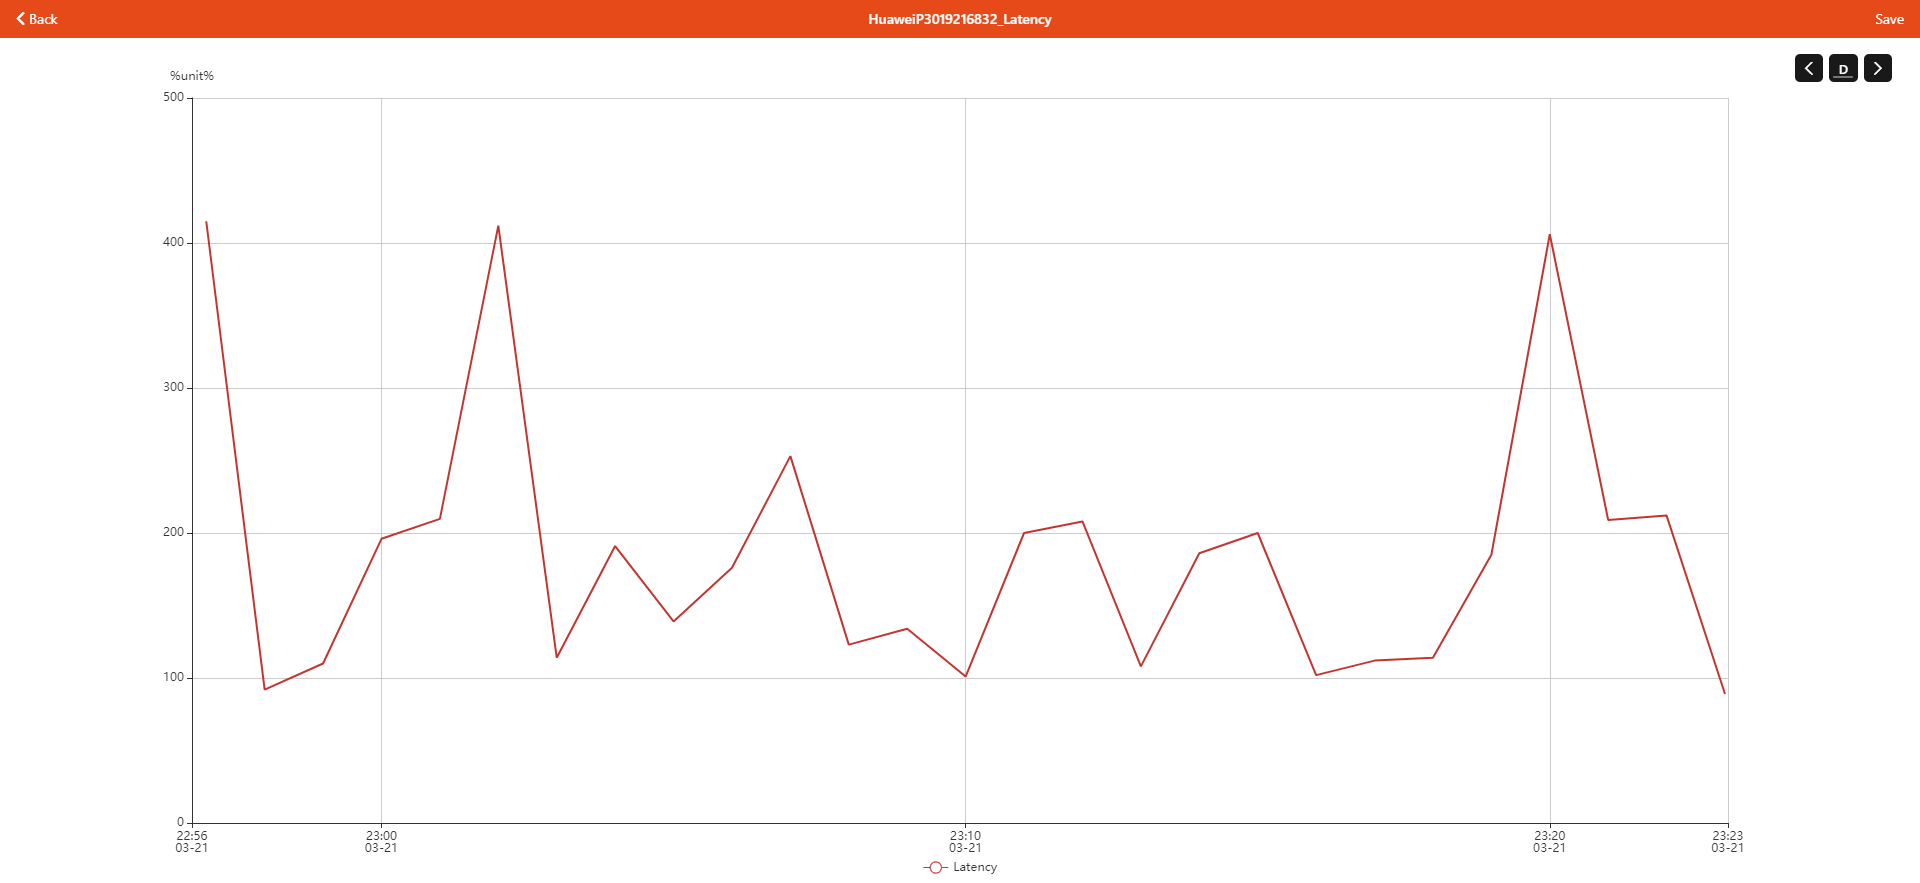
\includegraphics[width=0.9\linewidth]{figures/PersistenceExample.png}
  \caption{Persistence example: Latency value for accessing a remote device (in ms). }
  \label{fig:PersistenceExample-figure}
\end{figure}

\section{Device visualization and real-virtual world location mapping}

Each of the IoT devices is visualized through widgets in the platform, but the creation of widgets for 3D-modeling requires additional time. Если уже существует 3D-модель устройства, то разрабочик может ее добавить в платформу в качестве виджета, а затем соединить с дополнительными виджетами.

Но очень часто при разработке новых устройств еще не создана 3D-модель устройства, или в used IoT environment многие устройства также еще не имеют соответствующих 3D-моделей. Существует несколько решений данной проблемы. Первое решение - это использование 3D-моделей аналогичных устройств. Тем не менее, не всегда получается найти необходимую модель, или качество данных моделей не соответствует требованиям. Второе решение - это сканирование устройств. С помощью 3D сканеров, основанных на камерах глубины, уже возможно сканирование вещей с приемлемой точностью, тем более по относительно доступной цене. Если необходима миллиметровая точность сканирования, то можно использовать дорогостоящие профессиональные решения.

Полученные Widgets of 3D-models добавляются в виртуальную реальность. In case of NUIX-Studio App, scenes representing different environments are used. An example scene is demonstrating a smart home environment. Тем не менее, возможно использование также множества других сцен. Сцены можно создавать самому внутри редакторы Unity, а также с помощью Things Constructor, принимая окружающие объекты за виджеты (например, положение людей на улице представлено в виде Items of Location type). Такой подход занимает довольно длительное время, тем более, если существует необходимость использовать копию реального окружения в виртуальной реальности. Чтобы сократить время моделирования, можно использовать такие решения, как 3D-сканирование окружение. Уже сейчас доступно сканирование окружения с хорошей точностью на большом количестве различных смартфонов с помощью Depth Lab from Google, а также с отличной точностью на iPhone 12 Pro с помощью систем разработки Apple. Тем не менее, данные сканы окружения представляют из себя статические сцены. Если внутри данного окружения переместить объект, то скан придется выполнять заново. К сожалению, на данный момент не существует решения данной проблемы. Тем не менее, в следующей главе будет показано, что платформу можно адаптировать для работы с дополненной реальностью, что позволит избавиться от необходимости полного соответствия реального мира виртуальному.

Для отслеживания перемещения реальных IoT устройств в реальном мире могут быть использованы различные девайсы, такие как Bluetooth-метки, QR-коды, магнитные поля и т.д. Разработчикам предоставляется доступ к изменению положения каждого виджета. Таким образом, при изменении положения устройства в реальном мире, положения виджетов утсройства в виртуальном мире так же поменяется. При этом возможно провести и обратное действие, но для этого необходимо устройство, которое будет перемещать IoT девайсы в релаьности.

\section{Physics support}

С переносом ресурсоемких вычислений на отдельный сервер появляется возможность производить более достоверную симуляцию физических объектов. Такие вычисления, как обработка освещения, звука, и других волн различных диапазонов, а также различных веществ, таких как газ, вода, лишь ограничены алгоритмами.

\section{Scalability}

Когда количество Widgets внутри системы возрасает, производительность платформы остается на примелемом уровне. Благодаря тому, что каждому виджету ставится в соответствие некоторый уникальный id, время обращения к конкретному виджету составляет O(1) опреаций. Event processing time takes O(n) operations, where n is the number of connected widgets. It is theoretically impossible to reduce the complexity for processing an event since every Widget has to be accessed. In this case, the event processing time is linearly dependent on the number of Widgets connected to the Item. В общем же, можно сказать что общая производительность платформы также линейно зависит от количества IoT devices in the environment.

\section{Review}
Таким образом, было показано, что архитектура платформы позволяет поддерживать все возможные устройства, создавать новые устройства из существующих и помещать их в реальный мир. Платформа позволяет эффетктивно обрабатывать запросы от неограниченного числа устройств.

Тем не менее, архитектура платформы не позволяет обойти ограничения, связанные с некоторыми теоретическими расчетами. Тем не менее, для того, чтобы обойти данные ограничения, можно использовать платформу внутри дополненной реальности, о чем будет рассказно в следующей главе.